% Chapter Template

\chapter{Visualising real-world networks} % Main chapter title

\label{Chapter6} % Change X to a consecutive number; for referencing this chapter elsewhere, use \ref{ChapterX}

Add 4 questions as relevant for this chapter
Talk about this chapter structure
What this chapter does in each section

\section{Generating diagrams of the real-world}   
To begin to analyse the differences between the emulated Serval networks and those of real-world networks, identical Serval networks are to be run in both emulation using the test framework and in the real world.
By using the tools created throughout this thesis, the differences and similarities in the functionality of the networks can be analysed.
Of particular use will be the generation of diagrams as implemented in Chapter 5.
To do this however, some changes will need to be made to the program to support the generation of real-world Serval tests.
The first of these is that initial log files will need to be made for the real-world tests.
This log file is simply a single compiled file of the logs in the real-world tests that the program will use as the input to generate the simple log file and the diagrams.
Additionally, some mild changes will need to be made to the program. 
These changes should be relatively minor: move to using just LBARD for the generation of radio major events since real-world tests don't use Fakeradio, and retrieve node SIDs from Servald since we can not use the SIDs reported by the test framework.

The reasoning behind why the program is so well-suited to handling real-world events is due to the nature of the test framework: the test framework runs real Serval software, with the only part that is not present in real-world scenarios being that of Fakeradio.
If solutions to these changes are found that exist solely within Servald or LBARD, then these solutions will be portable to analysis of both the emulated test framework and real-world tests.

\subsection{Creating initial log file}
To create the initial log file to be used for real-world tests, multiple log files will need to be manually combined to create the single initial log file that the program requires.
This log file will simply contain all the log outputs from the Servald and LBARD processes that are involved in the real-world test.

This log file needs to follow the same format as that of the log files:
\begin{itemize}
    \item Four lines detailing the name, result, and start and finish time for the test
    \item Each LBARD process with a line proceeding each process listing which LBARD process it is
    \item Each Servald process with a proceeding line detailing which Servald process it is
\end{itemize} 

Additionally, the SIDs for each of the nodes will need to be listed at the top of the file. 
This is because as the initial log file is processed, any references to a SID involve a lookup to determine which node this is referring to, as such these SIDs need to be listed in advance.
For emulated tests this is not necessary, as these SIDs are reported by the test framework at the beginning of the log file.
A combined real-world log file may look similar to \figurename{ \ref{fig:chapter6RealWorldLog}}.

\begin{figure}
    \begin{centering}
\begin{lstlisting}[basicstyle=\small, breaklines, frame=single]
Name:     FieldTest
Result:   PASS
Started:  2020-08-24 13:22:55.044
Finished: 2020-08-24 13:23:32.497
++++++++++ fork[1] %lbardA log.stdout ++++++++++
469:My SID as hex is [SID]
++++++++++ fork[1] %lbardB log.stdout ++++++++++
469:My SID as hex is [SID]
++++++++++ fork[1] %lbardA log.stdout ++++++++++
[LBARD log file for node A]
++++++++++ fork[1] %lbardB log.stdout ++++++++++
[LBARD log file for node B]
#----- var/servald/instance/A/servald.log -----
[Servald log file for node A]
#----- var/servald/instance/B/servald.log -----
[Servald log file for node B]
\end{lstlisting}
        \caption{Example format of a compiled real-world log file with two nodes, A and B}
        \label{fig:chapter6RealWorldLog}
    \end{centering}
\end{figure}

Additionally, to ensure that real-world tests are producing the appropriate log output to create network diagram, every field test must have — at a minimum — some specific configurations.
For LBARD processes, the flags that must be set are:
\begin{lstlisting}
    bundles
    pieces
    announce
    message_pieces
    sync
    sync_keys
    \end{lstlisting}

With these flags, LBARD will produce the minimum log output required to generate diagrams. 
\todo{Add more info about what each of these does}

For Servald processes no specific configurations are required, however it is recommended to run each process with the following configuration as a minimum:
\begin{lstlisting}
set log.console.show_pid on 
set log.console.show_time on 
set debug.server on 
set debug.mdprequests on 
set debug.httpd on 
set debug.rhizome_manifest on
set debug.rhizome_sync_keys on
set debug.msp on
set debug.config on
set debug.mdprequests on
set debug.mdp_filter on
set debug.verbose on
\end{lstlisting}
These configurations will allow for a good coverage of Servald functionality, and provide the necessary information for a deeper analysis of real-world tests.


\subsection{Adding support for real-world tests}
Once the initial log file has been created for the real-world test, this can then be run through the program. \todo{We need a better name than just program}

\todo{Fix the tone here - authorative}
The program would produce a satisfactory simple log file based off of this real-world initial log file, however when any other form of output is run, such as the PDF diagram generation, the amount of major events produced is minor and only included Servald events.
This is due to the program's reliance on Fakeradio for determining major events.
For tests produced by the test framework this is perfectly reasonable; Fakeradio handles all the radio traffic and so it makes sense to use this.
However, real-world tests quite obviously do not require Fakeradio to handle the radio traffic, and as such no major events can be determined by analysing Fakeradio output as Fakeradio is never run.
As such, some other way of retrieving major events must be implemented.

Achieving this is relatively simple, if Fakeradio is not detected, every time a LBARD process announces it has sent a piece, simply use this as the basis of a major event.
An example of this log output can be seen in \figurename{ \ref{fig:chapter6RLBARDSent}}
This method has some drawbacks however, LBARD will only report that it is sending a bundle to a single node at a time and — as LBARD will prioritise pieces of bundles that multiple neighbour nodes require — this means that purely using this log output will not show multiple recipients of a bundle piece.
To mitigate this, the assumption will need to be made that LBARD is transmitting to all of its neighbours when it sends a bundle.
Despite this drawback, using the LBARD log output actually has an improvement: LBARD reports the start and end bytes of the piece it is sending.
By using these start and end pieces, a bundle bitmap can be developed, allowing for easier analysis of how LBARD is sending pieces through the network.

With these minor changes made, the compiled log files of the real world tests can then be run through the program, and any form of output — including diagram generation — should work without issue.


\begin{figure}
    \begin{centering}
\begin{lstlisting}[basicstyle=\small, breaklines]
    >>> [13:13.02.983 662D*] I just sent manifest piece [0,128) of [BID] for [receiving SID]
\end{lstlisting}
        \caption{LBARD output when sending a bundle piece}
        \label{fig:chapter6RLBARDSent}
    \end{centering}
\end{figure}


\subsection{Displaying bundle bitmaps}
To assist with the analysis of LBARD sending and receiving bundles and bundle pieces, bundle bitmaps can be used to display the count of times that a specific section of a bundle body or manifest has been sent to a node.
This is particularly useful when analysing LBARD networks, as a long-standing bug in LBARD revolves around bundles not being properly marked as received \todo{reference}.
By analysing these bundle bitmaps, Serval testers will be able to easily determine what pieces of a bundle have been sent excessively or not at all.

\subsubsection{Calculating bitmap partitions}
The bitmap partitions are simply the byte borders that a node receives for this bundle.
For instance, a node may receive bytes 0 to 64 in one transfer, and bytes 65 to 256 in the next.
Then, assuming that these are the only transfers that this node receives for this bundle, the partitions would be 0, 64, and 256.

Calculating the bitmap partitions is simple; every time LBARD reports it sends a bundle piece, add the start and end byte values to an array for each of the destination nodes.
The end result of this is that at the conclusion of the processing of the simple log file, each node has an array of bitmap partitions for every bundle that was sent during the test.
For some nodes who were never sent a bundle, this array may be empty, however for other nodes this will contain every single partition value that it received from 0 to the end byte value.

While this will produce an accurate view of the pieces that a node has been sent throughout the test, this does not provide an adequate level of granularity.
With the exception for the last piece, bundle pieces always have a granularity of 64 bytes \todo{ref}, however LBARD often attempts to send pieces in 128 byte increments. 
Thus, to account for this necessary level of granularity, the program must add any non-existent bundle partitions that are a multiple of 64 and less than the maximum byte value that this node has received.
To do this, the program iterates through the sorted array of byte partitions, and if any multiple of 64 is missing from where it should be in the array, appends it to the end.
After it iterates through the array, the program sorts the array, giving a complete bundle bitmap for both the body and manifest with a granularity of 64 bytes (excluding the last piece which may be less than 64 bytes).


\subsubsection{Displaying bitmaps}
Once the bitmap partitions had been calculated for every node, the bitmaps can then be displayed.
To display these, both the partitions and a current count of the number of times each partition has been sent to the specified node must be known.
This is because the bitmaps are displayed alongside each major event of an LBARD transfer in both the ASCII and PDF outputs. 
As these bitmaps are related to a LBARD major event, the count of sent bundle pieces must accurately represent the number of times this piece has been sent \emph{as of the time of the major event}.

To display the current bitmap partition count during the ASCII or PDF output, every time a LBARD transfer is encountered, each of the receiving nodes of this bundle transfer have their bitmap counts adjusted.
What this means is that the program uses the message type (body or manifest) and the start and end bytes of the message and increments the count of every partition for that node for that bundle between the start and end bytes.
The end result of this is that every time LBARD reports that it sends a bundle piece — for example, a body piece of bytes 64 to 192 of BID ABCDE1234* — then for every receiving node of this message, the count for each partition between bytes 64 to 192 are incremented by one for that specific bundle ID.

With this, a 'live' bitmap of each of the bundles can be displayed for each of the receiving nodes at the time of the major event.
Displaying this in the ASCII mode is simple, whenever a major event is encountered where LBARD sends bundle pieces, simply adjust the count using the known BID and start and end byte values of this event, and then iterate through every receiving node and print the count of each of the partitions. 
This can be seen in \figurename{ \ref{fig:chapter6ASCIIPartition}}.

\begin{figure}
    \begin{centering}
\begin{lstlisting}[basicstyle=\small, frame=single, breaklines]
57: [ 13:22:54.982] Sent body piece [0,50) of 5B59E446*
A -> BCD
  Manifest Bitmap (B):
  | [0,64)    | [64,128)  | [128,192) | [192,256) |
  | 1         | 1         | 1         | 1         |
  Body Bitmap (B):
  | [0,50)     |
  | 2          |
  
  Manifest Bitmap (C):
  | [0,64)    | [64,128)  | [128,192) | [192,256) |
  | 1         | 1         | 1         | 1         |
  Body Bitmap (C):
  | [0,50)     |
  | 2          |
  
  Manifest Bitmap (D):
  | [0,64)    | [64,128)  | [128,192) | [192,256) |
  | 1         | 1         | 1         | 1         |
  Body Bitmap (D):
  | [0,50)     |
  | 2          |
\end{lstlisting}
        \caption{ASCII representation of bundle count}
        \label{fig:chapter6ASCIIPartition}
    \end{centering}
\end{figure}


For the PDF output, the bitmap partition and counts are displayed in a table underneath the network topology diagram.
The program creates two tables per receiving node, one for body and one for manifest bitmaps.
These tables simply list the start and end bytes for each partition in the header row, and beneath each of these, show the 'live' count of the number of times that these partitions have been sent.
This can be seen in \figurename{ \ref{fig:chapter6PDFPartition}}.

\begin{figure}
    \begin{centering}
        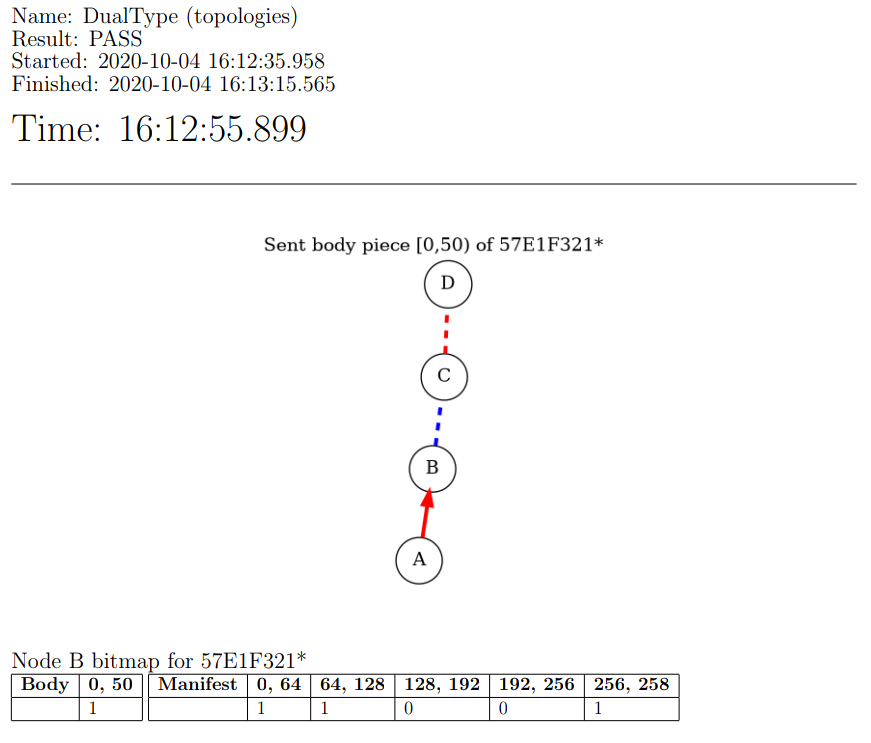
\includegraphics[width=15cm,height=20cm,keepaspectratio]{Figures/Chapter6-PDFPartition.png}
        \caption{PDF Output showing network diagram and bundle bitmap}
        \label{fig:chapter6PDFPartition}
    \end{centering}
\end{figure}

\section{Comparing real-world and framework tests}
\begin{itemize}
    \item Number of bundle bitmaps by the time that all bundles are sent
    \item General behaviour
    \item "simulation fidelity", i.e., is the simulation able to reproduce known real-world problems.
    \item Multi hop communications aren't working properly but do in simulation
    \item Lack of bundle background things
    \item No visibility to see what is happening
    \item Diagnostic power - how effective the simulation framework is for revealing the cause rather than revealing them \todo{Talk about in lit review}
\end{itemize}




\section{Summary}
\begin{itemize}
    \item Summarise what this chapter did
    \item Talk about why it was important
    \item Link to next section
\end{itemize}
\textbf{Summarise this section and link with results}